\cleardoublepage

\chapter{Antecedentes}
\label{Cap2:Antecedentes}

El principal objetivo de este apartado es exponer brevemente al lector las bases, tanto matemáticas como físicas, para poder entender y trabajar con propiedades metamórficas y en particular, su aplicación a la computación cuántica. Para ello, vamos a hacer un breve repaso a conceptos básicos de álgebra lineal en matemáticas, los postulados de la mecánica cuántica y una iniciación a la computación cuántica y el testing metamórfico. 

\vspace{5pt}
Esta sección, que podría ser una simple continuación de la introducción, va a ser más extensa de lo que se podría esperar. Ya que para trabajar de forma cómoda, sobre el tema a tratar, necesitamos un salto en conocimientos que se han tenido que adquirir.

\section{Introducción matemática}
\label{Sec2.1:Matematicas}
Para poder desarrollar y entender la mecánica cuántica, que presentaré a continuación, la programación cuántica y en particular, sus algoritmos, vamos a necesitar cierta base matemática y de notación. Quizás, las definiciones que siguen este párrafo pueden parecer aleatorias, aunque todo cobrará sentido conforme vayamos profundizando en la mecánica y programación cuántica.

\vspace{5pt}

Definimos un \textbf{espacio de Hilbert}, $\mathscr{H}$, como un $\mathbb{C}$-espacio vectorial dotado de un producto interno que es completo. En particular, como vamos a tratar solo $\mathbb{C}$-espacios vectoriales con producto interno finito, este será completo.

\vspace{5pt}

Por el \textbf{Teorema de representación de Riesz}, tenemos que $\mathscr{H}$ es anti-isomorfo a $\mathscr{H}^{*}$, por ser $\mathbb{C}$ nuestro cuerpo base.

\vspace{5pt}

Denotaremos como ket, $|v\rangle$, a un vector $v$ de $\mathscr{H}$. Análogamente, a toda transformación $w$ de $\mathscr{H}^{*}$, la denotaremos como bra, $\langle w|$. Esta notación es conocida como \textbf{notación de Dirac} y será utilizada en mecánica cuántica.

\newpage

Veamos ahora distintas definiciones para operadores:
\begin{itemize}
    \item Sea $\mathscr{A}:\mathscr{H} \rightarrow \mathscr{H}$ continuo, se denomina \textbf{adjunto del operador lineal} $\mathscr{A}$ al único operador   $\mathscr{A}^{*}:\mathscr{H} \rightarrow \mathscr{H}$ talque $<\mathscr{A}v,w>$ = $<v,\mathscr{A}^{*}w>$.
    \item Se dice que $\mathscr{A}:\mathscr{H} \rightarrow \mathscr{H}$ es un \textbf{operador autoadjunto} si $\mathscr{A}$ = $\mathscr{A}^{*}$. Por lo cual los autovalores de $\mathscr{A}$ son reales.
    \item Llamaremos matriz \textbf{hermitiana} a la matriz $A$ que determina el operador autoadjunto $\mathscr{A}$. De aquí obtenemos que $A^{*}$ es la traspuesta conjugada de $A$.
    \item Se dice que $\mathscr{U}:\mathscr{H} \rightarrow \mathscr{H}$  continuo, es \textbf{unitario} si $<v,w>$ = $<\mathscr{U}v,\mathscr{U}w>$, que en particular es invertible.
\end{itemize}

\vspace{5pt}

Para finalizar con esta sección vamos a ver una manera de combinar dos espacios vectoriales, en particular, dos espacios de Hilbert que nos permitirá unir dos sistemas cuánticos, esta operación es el producto tensorial.\cite{B:Nielsen:2002} \footnote{\url{https://es.wikipedia.org/wiki/Producto_tensorial}}

\vspace{10pt}

Sean $\mathscr{H}$ y $\mathscr{H}'$ dos espacios de Hilbert,

\vspace{5pt}
\begin{equation}
    F(\mathscr{H} \times \mathscr{H}') = \left\lbrace \sum_{i=1}^{n}z_{i} (h_{i},h_{i}')\:|\:n \in \mathbb{N},\: z_{i} \in \mathbb{C},\:(h_{i},h_{i}') \in \mathscr{B}(\mathscr{H} \times \mathscr{H}') \right\rbrace
\end{equation}

\vspace{5pt}
\begin{equation}
\begin{split}
    \mathscr{R} =  (h_{1}+h_{2},h') \sim (h_{1},h') + (h_{2},h') \\ 
    (h,h_{1}'+h_{2}') \sim (h,h_{1}') + (h,h_{2}') \\
    z(h,h') \sim (z h,h') \sim (h,z h')
\end{split}
\end{equation}

\vspace{5pt}
Definimos el \textbf{producto tensorial} de $\mathscr{H}$ y $\mathscr{H}'$ , $\mathscr{H} \otimes \mathscr{H}'$, como el espacio cociente entre $F(\mathscr{H} \times \mathscr{H}')$ y $\mathscr{R}$, es decir, $\mathscr{H} \otimes \mathscr{H}' = F(\mathscr{H} \times \mathscr{H}')/\mathscr{R}$. Partiendo directamente desde la definición de la relación obtenemos:

\begin{itemize}
    \item \textbf{Linealidad}: Sea $z\in\mathbb{C}$, $|h\rangle\in\mathscr{H}$ y $|h'\rangle\in\mathscr{H}'$. Entonces:
        \begin{equation}
            z\:(|h\rangle \otimes |h'\rangle) = (\:z|h\rangle) \otimes |h'\rangle = |h\rangle \otimes (\:z|h'\rangle)
        \end{equation}
        
    \newpage
    \item \textbf{Asociatividad}:
    \begin{itemize}
        \item Sea $|h_{1}\rangle\in\mathscr{H}$, $|h_{2}\rangle\in\mathscr{H}$ y $|h'\rangle\in\mathscr{H}'$. Entonces:
            \begin{equation}
                (|h_{1}\rangle + |h_{2}\rangle)\otimes|h'\rangle = |h_{1}\rangle \otimes|h'\rangle + |h_{2}\rangle \otimes|h'\rangle
            \end{equation}

        \item Sea $|h\rangle\in\mathscr{H}$, $|h_{1}'\rangle\in\mathscr{H}'$ y $|h_{2}'\rangle\in\mathscr{H}'$. Entonces:
            \begin{equation}
                |h\rangle \otimes (|h_{1}'\rangle) + |h_{2}'\rangle) = |h\rangle \otimes|h_{1}'\rangle + |h\rangle \otimes|h_{2}'\rangle
            \end{equation}
    \end{itemize}
\end{itemize}

Además alcanzamos los siguiente resultados sobre el producto tensorial:
\begin{itemize}
    \item \textbf{Base}: $|i\rangle \otimes |j\rangle$ es una base de $\mathscr{H} \otimes \mathscr{H}'$ donde $|i\rangle$ y $|j\rangle$ pertenecen a una base ortonormal de $\mathscr{H}$ y $\mathscr{H}'$ respectivamente. 
    
    \item \textbf{Producto interno}: los productor internos de $\mathscr{H}$ y $\mathscr{H}'$ inducen naturalmente un producto interno en $\mathscr{H} \otimes \mathscr{H}'$ por lo que hereda la estructura y con ella, las nociones de adjunta, unitaria, normalidad y hermiticidad.
    
    \item \textbf{Producto de Kronecker}, se corresponde con el producto tensorial de aplicaciones lineales. Nos será de gran utilidad a lo largo de este trabajo y nos ayuda a visualizar el producto tensorial. Veamos un ejemplo, si $A$ y $B$ son 2 matrices, entonces:\newline

        \begin{equation}
        A\otimes B = \begin{bmatrix}
        a_{11}B & a_{12}B & ... & a_{1n}B\\
        a_{21}B & a_{22}B & ... & a_{2n}B\\
        \vdots & \vdots & \ddots & \vdots\\
        a_{m1}B & a_{m2}B & ... & a_{mn}B
        \end{bmatrix}
        \end{equation}

    Además, si $A$ y $B$ unitarias, entonces $A\otimes B$ es unitaria.

    \vspace{5pt}
    \item \textbf{Dimensión}: $dim(\mathscr{H} \otimes \mathscr{H}')=dim(\mathscr{H})\cdot dim(\mathscr{H}')$
\end{itemize}

Estos dos últimos apartados nos muestran la complejidad que vamos a tener a la hora de realizar cálculos, ya que la dimensión de las matrices va a crecer de manera exponencial.

\newpage

\section{Introducción cuántica}
\label{Sec2.2:Fisica}

La base principal para el comienzo de la computación cuántica fue el desarrollo de la física cuántica. Para poder entender mejor que variaciones e implicaciones tiene, vamos a ver los postulados de la mecánica cuántica y sus diferencias con la mecánica Newtoniana. Aquí encontrará sentido la base matemática presentada en la \hyperref[Sec2.1:Matematicas]{sección 2.1}.

\vspace{5pt}

Para empezar, en mecánica clásica, un sistema de N partículas queda definido por un vector en un espacio $\mathbb{R}^{3N} \times \mathbb{R}^{3N}$ donde las primeras coordenadas definen la posición y las últimas la velocidad. La evolución de este sistema se rige por la segunda Ley de Newton que relaciona la fuerza con la aceleración y la masa.

\vspace{5pt}

Por otra parte, en física cuántica, el estado y evolución de un sistema viene determinado por sus postulados\cite{B:Nielsen:2002}\cite{Note:Martin} que veremos a continuación \footnote{\url{https://en.wikipedia.org/wiki/Mathematical_formulation_of_quantum_mechanics\#Postulates_of_quantum_mechanics}}, así como una de las posibles interpretaciones que cada uno podría tener. Estos postulados nos ayudaran posteriormente a fijar la base de nuestros programas cuánticos.
\vspace{10pt}

\textbf{Postulados cinemáticos o de representación:}
\begin{itemize}
    \item \textbf{Primer postulado:}\label{Postulado1} El estado en un sistema aislado, en un instante t, se corresponde con $| \varphi (t) \rangle$, en un espacio de Hilbert, $\mathscr{H}$.
    
    \item \textbf{Segundo Postulado:}\label{Postulado2} El espacio que representa un sistema compuesto es el producto tensorial del los espacios de cada componente del sistema. Es decir, si tuviéramos n componentes, el espacio total sería $|\varphi_{1}\rangle \otimes |\varphi_{2}\rangle \otimes \dotsi \otimes |\varphi_{n}\rangle = |\varphi_{1}\varphi_{2}\dotso \varphi_{n}\rangle$, de forma notacional.
\end{itemize}

\textbf{Postulados dinámicos:}
\begin{itemize}
    \item \textbf{Tercer postulado:}\label{Postulado3} Evolución determinista.
        \begin{itemize}
            \item \textbf{Primer apartado}:\label{Postulado3.1} La evolución de un vector $| \varphi (t) \rangle$ está determinada por la ecuación de Schrödinger, $\imath \hbar \dfrac{d|\varphi\rangle}{dt}=H |\varphi\rangle$. Donde H es el Hamiltoniano del sistema, que es un operador hermitiano. Además se entiende H(t) como un observable asociado a la energía total del sistema.
            \item \textbf{Segundo apartado}:\label{Postulado3.2} La evolución de un sistema aislado se describe por una transformación unitaria del estado inicial. $| \varphi (t) \rangle = U(t;t_{0})  | \varphi (t_{0}) \rangle$.
        \end{itemize}
    
    \vspace{5pt}
    \newpage
    \item \textbf{Cuarto postulado:}\label{Postulado4} Evolución probabilística, tenemos observador.
    \begin{itemize}
        \item \textbf{Primer apartado}:\label{Postulado4.1} Cada medida $\mathscr{A}$ esta descrita por un operador hermitiano A que actúa sobre $\mathscr{H}$, decimos que este operador es observable, debido a que sus autovectores forman una base de $\mathscr{H}$. El resultado de medir una cantidad $\mathscr{A}$ debe ser uno de los autovalores correspondientes al observable A.
        \vspace{5pt}
        \item \textbf{Segundo apartado}:\label{Postulado4.2} $Prob(\lambda_{i}) =  \dfrac{||\:P_{|v_{i}\rangle} | \varphi (t) \rangle\:||^{2}}{||\:| \varphi (t) \rangle\:||^{2}} = \dfrac{|\: \langle  v_{i}  |\: \varphi (t)  \rangle\:|^{2}}{||\:| \varphi (t) \rangle\:||^{2}}$
        \vspace{5pt}
        \item \textbf{Tercer apartado}:\label{Postulado4.3} Si tras realizar una medición $\mathscr{A}$ del estado $|\varphi(t) \rangle$ da como resultado $a_{n}$, entonces el estado del sistema colapsa a la proyección normal de $|\varphi(t) \rangle$ en el subespacio de autovectores asociado a $a_{n}$,  $P_{|v_{n} \rangle} | \varphi (t) \rangle$.
    \end{itemize}
\end{itemize}

Todos estos postulados van a ser clave en los distintos aspectos de la computación cuántica, como la definición del sistema más simple como el \textit{qubit}.

\vspace{10pt}
\section{Programación cuántica, Qiskit}
\label{Sec2.3:Qiskit}

 La programación cuántica se basa en la creación de un circuito o algoritmo cuántico, normalmente representado geométricamente, donde se realizan operaciones (operadores unitarios) sobre los distintos qubits, así como sus mediciones\cite{B:QuantumScientist:2008}.

 \vspace{8pt} 

 Para realizar nuestros programas cuánticos y simulaciones nos vamos a apoyar en \textit{Qiskit}, es un paquete de desarrollo libre creado por IBM para crear y manipular programas cuánticos así como realizar simulaciones\footnote{\url{https://qiskit.org/}}. Ya sean teóricas o conectando nuestros programas con los ordenadores cuánticos de IBM. Esto nos dará unos resultados más realistas donde podremos apreciar el ruido que hay actualmente en estos ordenadores.

 \vspace{8pt} 
 
 Se programará en Qiskit, una libreria de Python, en el que se permite definir y utilizar los circuitos. Además, para una mejor visualización de lo que representa el código utilizaré jupyter notebook. Otra opción sería generar los circuitos de forma geométrica en IBM \footnotemark[1].

 \vspace{8pt} 

 Además, exisitirían otras opciones como \textit{Azure Quantum}\footnote{\url{https://azure.microsoft.com/en-us/services/quantum/}} en \textit{C\#} de Microsoft, \textit{Cirq}\footnote{\url{https://quantumai.google/cirq}} en \textit{Python} de Google o \textit{Pyket}\footnote{\url{https://cqcl.github.io/tket/pytket/api/index.html}} también en \textit{Python} entre otros. \newline
 
 Como mencionamos anteriormente los postulados cuánticos, ordenados de acorde a la utilización en este texto, nos van a permitir sentar las bases de la computación cuántica, el primer ejemplo es el qubit. \newline
 
 Si recordamos el \hyperref[Postulado1]{postulado 1} de la mecánica cuántica, vamos a definir \textbf{qubit} como el sistema cuántico más simple, que va a ser nuestra base en la programación cuántica. Un \textbf{qubit} es un espacio bidimensional, donde vamos a suponer que tomamos la base ortonormal $|0 \rangle = \begin{bmatrix} 1\\0 \end{bmatrix}$ y $|1 \rangle = \begin{bmatrix} 0\\1 \end{bmatrix}$. De aquí podemos obtener la combinación lineal de cualquier vector de estado del qubit, aunque los vectores de estado deben de cumplir la condición de normalización, es decir, si $|\varphi \rangle = a |0\rangle + b |1\rangle = \begin{bmatrix} a\\b \end{bmatrix}$ con $a,b \in \mathbb{C}$, entonces $|a|^{2}+|b|^{2}=1$. Esta condición se impone debido a que el cuadrado de los coeficientes determinan la probabilidad de aparición y por lo tanto la suma de todas la probabilidad de todas las posibilidades debe ser 1. Además, llamaremos estado de \textbf{superposición} a los estados del qubit que se encuentran en el continuo entre $|0\rangle$ y $|1\rangle$.\newline

 Estos estados de un qubit se entienden muy bien utilizando la \textbf{esfera de Bloch}, que observaremos en la Figura \ref{Fig:Bloch} \footnote{\url{https://en.wikipedia.org/wiki/Bloch\_sphere\#/media/File:Bloch\_sphere.svg}}. Debido a que si $|\Psi \rangle = a |0\rangle + b |1\rangle$, $|a|^{2}+|b|^{2}=1$. Podemos representar $|\Psi \rangle = e^{i\gamma}\left( cos\:\dfrac{\theta}{2} \:|0\rangle +\; e^{i\varphi}\;sin\:\dfrac{\theta}{2}\:|1\rangle\right)$, donde $\theta,\varphi,\gamma \in \mathbb{R}$. Si bien es cierto, podemos ignorar el factor $e^{i\gamma}$, ya que no tiene efectos observables. Hay que tener en cuenta que esta representación está limitada a un qubit, porque no hay manera simple de generalizarla.

  \begin{figure}[H]
    \centering
    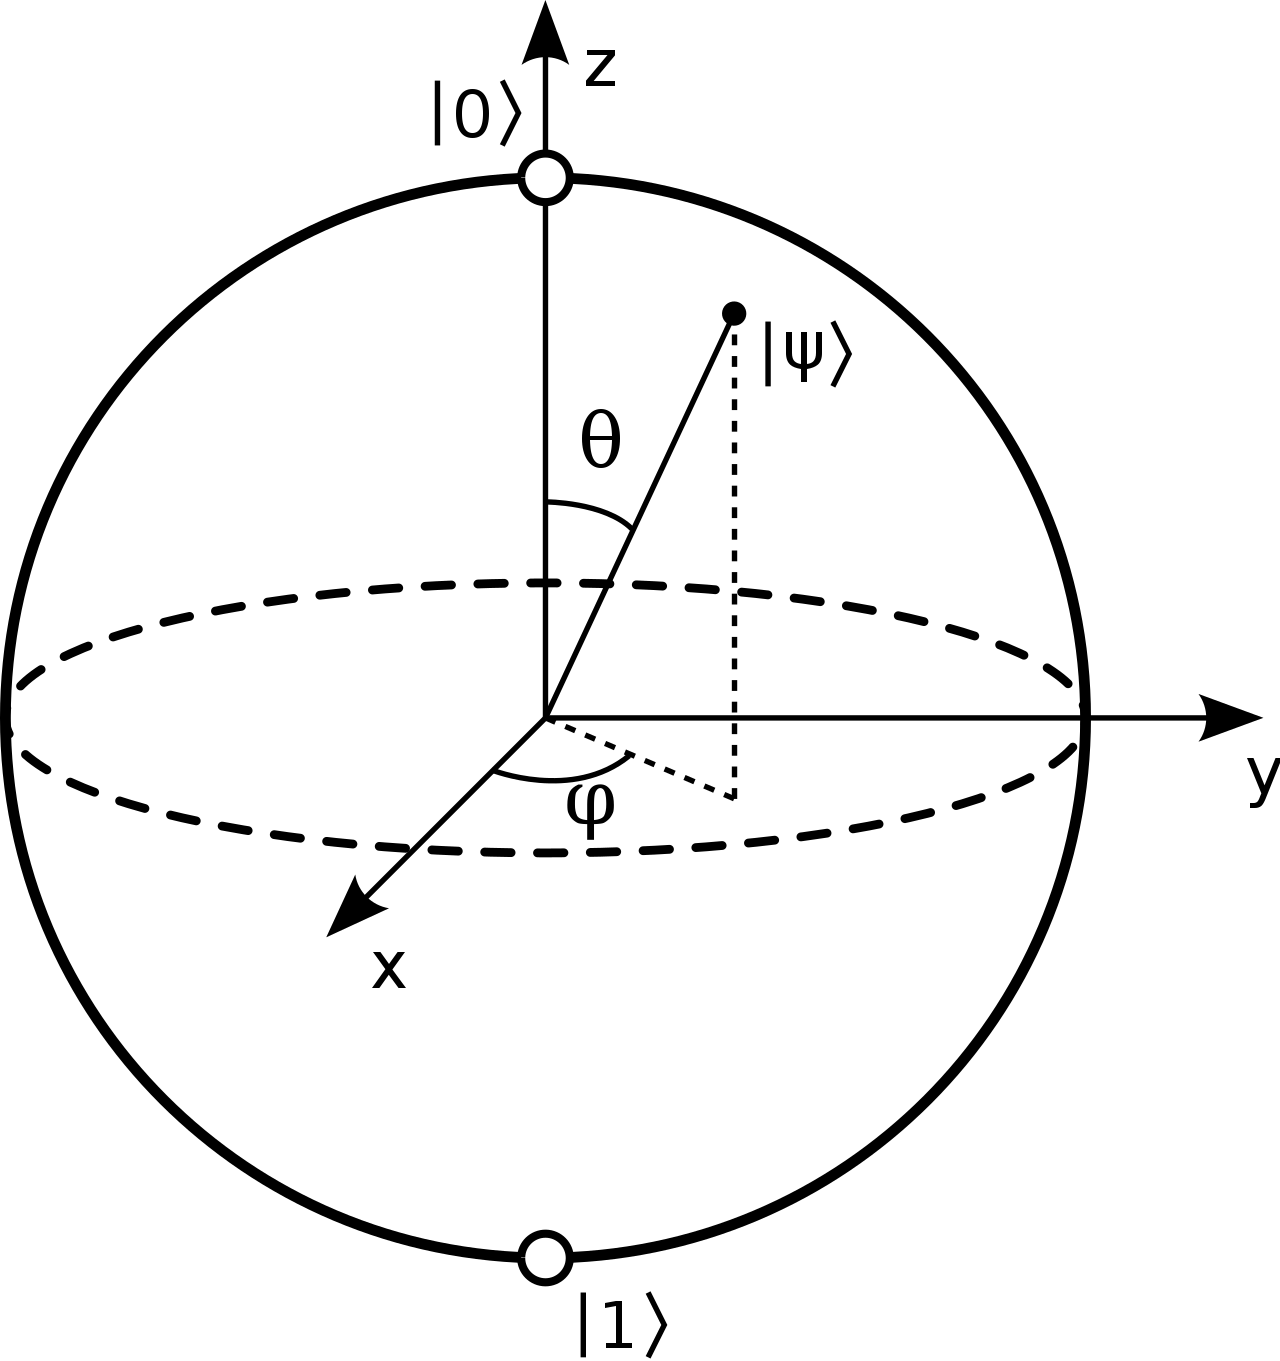
\includegraphics[width=0.37\textwidth]{TFG/imagenes/Bloch_sphere.png}
    \caption{Esfera de Bloch} 
    \label{Fig:Bloch}
  \end{figure}
 
 Veamos que es lo que ocurre ahora cuando en vez de un único qubit, tenemos varios y la relación que hay entre ellos. Para simplificarlo, tomemos el más simple, el sistema con 2 qubits. Si recordamos el \hyperref[Postulado2]{postulado 2} nos determinaba como interaccionaban estos dos qubits, como el sistema compuesto por ambos era su producto tensorial. Por ello, podemos definir el estado de un sistema de 2 qubits como:

    \begin{equation*}|\psi\rangle = a_{00}|00\rangle + a_{01}|01\rangle + a_{10}|10\rangle + a_{11}|11\rangle \;\;\text{donde}\; a_{00},\: a_{01}, \:a_{10}, \:a_{11} \in \mathbb{C}
    \end{equation*}

 A estos coeficiente complejos se les denomina \textbf{amplitud} de cada estado de la base. Al igual que ocurre en el qubit, $a_{00}+a_{01}+a_{10}+a_{11}=1$. Este resultado se puede obtener del producto de Kronecker, y además tendría sentido con la medición de las probabilidades. En este ejemplo se puede ver claramente que la dimensión de la base va a ser exponencial respecto al número de qubits.\newline
 
 Por último y antes de pasar a las puertas cuánticas y como operamos en el sistema, vamos a introducir un último concepto, el enredo cuántico o \textbf{\textit{entanglement}}. Esta es una propiedad de la mecánica cuántica que aparece en un sistema, se puede decir que un sistema de 2 qubits están en un estado de \textit{entanglement} cuando no es posible separar el estado como producto tensorial de los dos qubits\cite{B:QuantumScientist:2008}, diremos además que existe una correlación entre ellos. Normalmente se observa a la hora de hacer mediciones en dicho sistema, también conocido como \textit{entangled measurements}. Si bien es cierto, aún se sigue investigando esta propiedad, así como completar su teoría\cite{B:Nielsen:2002}.  Veamos un ejemplo simple que nos va a permitir obtener una idea. \newline

 Definimos $Bell\:state $ como $ \dfrac{|00\rangle + |11\rangle}{\sqrt{2}}$, veamos primero que no se puede expresar como producto tensorial. 

 \begin{equation*}
     (Bell\:state)\sqrt{2} = 1|00\rangle+ 0|01\rangle+ 0|10\rangle+ 1|11\rangle
 \end{equation*}
 
 \vspace{3pt}

 Suponemos que $(Bell\:state)\sqrt{2} = (a_{0}|0\rangle+a_{1}|1\rangle) \otimes(a_{0}'|0\rangle+a_{1}'|1\rangle)$, entonces:
 
 \vspace{3pt}
     
 \begin{center}
 $(a_{0}|0\rangle+a_{1}|1\rangle)\otimes(a_{0}'|0\rangle+a_{1}'|1\rangle) =a_{0}a_{0}'|00\rangle + a_{0}a_{1}'|01\rangle + a_{1}a_{0}'|10\rangle + a_{1}a_{1}'|11\rangle \Rightarrow$ \\ $\Rightarrow a_{0}a_{0}'=a_{1}a_{1}'=1$ y $a_{0}a_{1}'=a_{1}a_{0}'=0$
 \end{center}
 
 \vspace{3pt}

 Pero este sistema de ecuaciones no tiene solución, por lo que $(Bell\:state)\sqrt{2}$ no se puede expresar como producto tensorial y en particular, $Bell\:state$ tampoco.\newline
 
 Ahora queremos realizar una medición con base $\{|0\rangle,|1\rangle\}$, pero sabemos que sólo podemos obtener los resultados $|00\rangle$ o $|11\rangle$. Es decir, cuando se mida el primer qubit ya tendremos el valor del segundo sin haberlo medido \footnote{\url{https://jcc.dcc.fceia.unr.edu.ar/2006/slides/2006-diazcaro-samborskiforlese.pdf}}. Podemos encontrar otros ejemplos y preguntas muy interesantes sobre \textit{entanglement} en la \href{https://quantum-computing.ibm.com/composer/docs/iqx/guide/entanglement}{página de IBM}, donde estudia distintas posibilidades con la puerta CNOT, que presentaremos a continuación, y estados interesantes como \textit{Bell state}, \textit{GHZ states} and \textit{W states}.\newline

 Otro de los resultados interesantes es el Teorema de no Clonación, por el cual nos indica que no podemos copiar el estado de un qubit desconocido a otro qubit. Esto se puede entender, ya que si observáramos el qubit estaríamos realizando una medición y el estado colapsaría.\newline

 \textbf{Teorema 2.1 (No clonación)} \cite{B:Nielsen:2002}: Sea $\mathcal{H}$ un espacio de Hilbert en $\mathbb{C}$ y sean $|\varphi\rangle, |\psi\rangle \in \mathcal{H}$. Entonces, $\nexists U$ unitario sobre $\mathcal{H}\otimes\mathcal{H}$ talque $U|\varphi\rangle|\psi\rangle=|\varphi\rangle|\varphi\rangle$.\footnote{\url{https://es.wikipedia.org/wiki/Teorema_de_no_clonaci\%C3\%B3n}}


\subsection{Puertas y circuitos cuánticos}

 Partimos ahora del tercer postulado, en particular el \hyperref[Postulado3.2]{apartado 2}. Se podría ver que existe una correspondencia 1 a 1 entre el Hamiltoniano $H$, por ser hermitiano, y un operador unitario $U$. Estos operadores unitarios serán nuestras \textbf{puertas cuánticas} que vamos a usar junto a los qubits. Este postulado viene de la evolución \textbf{determinista} desde un puesto de vista dinámico, donde no se realiza ninguna observación sobre el sistema. Uno de los puntos importantes de que estos operadores sean unitarios es que conservan la norma, por lo cual no rompen la condición de normalización de la definición de qubit. \newline
 
 En programación cuántica estos operadores unitarios pueden crearse directamente con una matriz, que cumpla las condiciones necesarias, aunque habitualmente utilizaremos puertas cuánticas, operadores, especificas que son las utilizadas en los ordenadores cuánticos reales\cite{Note:Martin}. Veamos cuales son las puertas cuánticas mas útiles para un qubit:\cite{B:Nielsen:2002} \footnote{\url{https://en.wikipedia.org/wiki/Quantum_logic_gate}}

 \begin{itemize}
    \item \textbf{Puertas de Pauli}: Estas puertas son la más básicas y nos van a permitir, a excepción de la identidad, realizar rotaciones de $\pi$ radianes dentro de las esfera de Bloch, cada una sobre el eje que indica su propio nombre. Las matrices que determinan estas puertas generan una base del espacio de matrices hermitianas 2x2.
    \begin{itemize}
    
        \item \textbf{Puerta identidad}: $I = \begin{bmatrix} 1 & 0\\0 & 1 \end{bmatrix}$, con puerta geométrica $\Qcircuit @C=1em @R=.7em {& \gate{I} &\qw}$
        
        \item $\boldsymbol Y$: La puerta $Y$,  $\Qcircuit @C=1em @R=.7em {& \gate{Y} &\qw}$ , viene determinada por la matriz \begin{math} Y = \begin{bmatrix} 0 & -i\\i & 0 \end{bmatrix}\end{math}
        \vspace{3pt}
        
        \item $\boldsymbol Z$: La puerta $Z$, $\Qcircuit @C=1em @R=.7em {& \gate{Z} &\qw}$ , viene determinada por la matriz \begin{math} Z = \begin{bmatrix} 1 & 0\\0 & -1 \end{bmatrix}\end{math}
        
        \item $\boldsymbol X$: La puerta $X$ es un operador que viene determinado por la matriz \begin{math} X = \begin{bmatrix} 0 & 1\\1 & 0 \end{bmatrix}\end{math}
        
        Esta puerta sería la análoga cuántica a la puerta NOT clásica y nos permite 
        
        \vspace{3pt}
        $|0\rangle \rightarrow |1\rangle$, $|1\rangle \rightarrow |0\rangle$, por lo que dado $|\varphi \rangle = a |0\rangle + b |1\rangle \Rightarrow X|\varphi \rangle = b |0\rangle + a |1\rangle$
        \vspace{3pt}

        Su puerta geométrica al realizar los circuitos será: $\Qcircuit @C=1em @R=.7em {& \gate{X} &\qw}$
        \vspace{5pt}
    \end{itemize}
    
    \item \textbf{Puerta de Hadamard}, $H$: Este operador viene determinado por $H = \dfrac{1}{\sqrt{2}} \begin{bmatrix} 1 & 1\\1 & -1 \end{bmatrix}$
    \vspace{3pt}
    
    Probablemente la puerta más interesante de todas, que nos permite poner el qubit en un estado especial, es más, dichas transformaciones sobre la base tiene su propia notación:

    \begin{center}
        
    $|+\rangle = H|0\rangle = \dfrac{|0\rangle + |1\rangle}{\sqrt{2}} \quad \quad \quad |-\rangle = H |1\rangle = \dfrac{|0\rangle - |1\rangle}{\sqrt{2}}$\end{center}

    A su vez, al igual que las matrices de Pauli, la matriz de Hadamard realiza una rotación de $\pi$ radianes, pero esta vez sobre el eje $(\hat{x} + \hat{z}) / \sqrt{2}$. Puerta:
    $\Qcircuit @C=1em @R=.7em {& \gate{H} &\qw}$
    
    \item \textbf{Puerta de cambio de fase}, $P(\theta)$: Esta puerta nos va a permitir realizar rotaciones de un ángulo $\theta$ sobre el eje $\hat{z}$. Y está determinada por $P(\theta) = \begin{bmatrix}1 & 0\\0 & e^{i\theta} \end{bmatrix}$. El nombre de esta puerta puede llevar a confusión, ya que mencionamos anteriormente que la fase no era observable, pero en ese caso nos referimos a la fase general del qubit. En este caso el cambio de fase se realiza sobre los ejes.\newline

    Casos particulares de puertas importantes:
    \begin{itemize}
        \item $P(\pi) = Z$. 
        \item $P(\pi/2) = S$, también conocida como puerta de fase, 
    $\Qcircuit @C=1em @R=.7em {& \gate{S} &\qw}$
        \item $P(\pi/4) = T$, $\Qcircuit @C=1em @R=.7em {& \gate{T} &\qw}$
    \end{itemize}
 \end{itemize}
 
 Análogamente, se puede definir las matrices de rotación para los distintos ejes. Y en general, vamos a definir la puerta de rotación sobre un eje cualquiera $\Hat{n}$, esta puerta queda determinada por $R_{\Hat{n}}(\theta) = cos \left(\dfrac{\theta}{2}\right)\:I - i\:sin\left(\dfrac{\theta}{2}\right)\left(n_{x}X + n_{y}Y + n_{z}Z\right) $ \newline

 La idea de introducir al lector con esta puerta de rotación, además de su utilidad, se debe a que nos va a permitir presentar el siguiente teorema. Como se mencionó anteriormente, cualquier matriz unitaria 2 x 2, puede definir un operador sobre un qubit, veamos que relación hay con las rotaciones. \newline
 
 \textbf{Teorema 2.2: Descomposición Z-Y para un único qubit}\cite{B:Nielsen:2002}: Sea $U$ un operador unitario sobre un qubit. Entonces, existen números reales $\alpha,\beta,\gamma$ y $\delta$ tal que:
 \begin{center}
     $U = e^{i\alpha} R_{z}(\beta)R_{y}(\gamma)R_{z}(\delta)$
 \end{center}

 Existe un resultado análogo para X-Y. Este teorema va a permitir descomponer cualquier operador unitario en estas rotaciones y así, los ordenadores cuánticos actuales, pueden procesar cualquier circuito independientemente de las diferencias entre puertas que componen el circuito cuántico y las puertas que dispone el ordenador.\cite{Note:Martin} \newline

 Veamos ahora las puertas más importantes para más de un qubit, en particular nos vamos a fijar en 2 y 3 qubits, para 2 utilizaremos la base $\{|00\rangle,\:|01\rangle,\:|10\rangle,\:|11\rangle\}$ y la análoga para 3 qubits.

 \begin{itemize}
     \item \textbf{CNOT}, también conocida como \textit{puerta de control Pauli-X}. Es un caso particular de las puertas de control sobre cualquier operador. En este caso, sobre la puerta X. \newline 
     Este operador viene determinado por la matriz, 
     
     \begin{equation*}
     CNOT = \begin{bmatrix} 1 & 0 & 0 & 0\\0 & 1 & 0 & 0\\0 & 0 & 0 & 1\\0 & 0 & 1 & 0 \end{bmatrix}=\begin{bmatrix} I & 0  \\ 0 & X \end{bmatrix}
     \end{equation*}
     
     La interpretación de esta puerta es que si el primer qubit es $|1\rangle$, realiza la operación $X$ sobre el segundo qubit. En general, podríamos definir la puerta controlada para un operador U, de forma análoga intercambiando $X$ por $U$.\newline 
     
     La representación de CNOT en un circuito es: 
     \raisebox{7pt}{$\;\;\;\;\;\;\Qcircuit @C=1em @R=.7em {\lstick{q_{1}}&  \ctrl{1} &\qw \\ \lstick{q_{2}} &\targ & \qw }$}. En general,\raisebox{10pt}{ $\;\;\;\;\;\;\Qcircuit @C=1em @R=.7em {\lstick{q_{1}}&  \ctrl{1} &\qw \\ \lstick{q_{2}} &\gate{U} & \qw }$}
     
     \item \textbf{SWAP}, o puerta de intercambio de qubits. Con notación \raisebox{7pt}{$\;\Qcircuit @C=1em @R=1em {&  \qswap &\qw \\ &\qswap \qwx & \qw }$} . La determinada,
     
     \begin{equation*}
     SWAP = \begin{bmatrix}
         1 & 0 & 0 & 0 \\ 0 & 0 & 1 & 0 \\ 0 & 1 & 0 & 0 \\ 0 & 0 & 0 & 1
     \end{bmatrix} \end{equation*}

     Hay que aclarar que esta puerta no copia los estados de los qubits, si no que los intercambia. Por lo que no contradice el teorma de no clonación introducido anteriormente.
     
     \item \textbf{Toffoli, CCNOT}. Puerta de control sobre 2 qubits $q_{1}, q_{2}$ aplicando la puerta X a $q_{3}$. \\ \\ Usaremos como notación \raisebox{12pt}{$\;\;\;\;\;\;\Qcircuit @C=1em @R=.7em {\lstick{q_{1}}&  \ctrl{1} &\qw \\ \lstick{q_{2}} &\ctrl{1} & \qw  \\ \lstick{q_{3}} & \targ & \qw}$} . Queda determinada por,
     
     \begin{equation*}
        CCNOT = \begin{bmatrix}
        I & 0 & 0 \\ 0 & I & 0 \\ 0 & 0 & X
        \end{bmatrix}
    \end{equation*}

     Esta puerta, al igual que CNOT, podría generalizarse para un operador unitario U.
 \end{itemize}

 Existe un concepto que se utiliza a menudo que es el de \textbf{conjunto de puertas universales}\footnote{\url{https://en.wikipedia.org/wiki/Quantum_logic_gate\#Universal_quantum_gates}}que se define como el conjunto de puertas al que toda operación unitaria se puede reducir. Aunque, esto teóricamente es imposible debido a que el número de puertas que se pueden construir es no numerable, y cualquier conjunto finito que definamos, si lo es. Para solucionar este problema, nos apoyamos en el teorema de \textit{Solovay–Kitaev} \footnote{\url{https://en.wikipedia.org/wiki/Solovay\%E2\%80\%93Kitaev_theorem}}, que garantiza que esta reducción se puede hacer de forma eficiente, es decir, aproximándola con la precisión necesaria. Los ejemplos más conocidos son:

 \begin{itemize}
     \item $\{R_{\hat{x}},R_{\hat{y}},R_{\hat{z}},P,CNOT\}$
     \item $\{CCNOT, H\}$
 \end{itemize}

 Esto se debe a que existen diversas relaciones entre las puertas que hemos presentado como por ejemplo, los subíndices indicarán a que qubit se aplican en caso de ser necesario:

 \begin{itemize}
     \item $ZX=iY=-XZ$
     \item $CNOT=exp\left( i\frac{\pi}{4}(I-Z_{1})(I-X_{3})\right)$
     \item $HZH=X$
     \item $SWAP=\dfrac{I\otimes I + X \otimes X + Y\otimes Y + Z\otimes Z}{2}$
     \item $CCNOT=exp\left( i\frac{\pi}{8}(I-Z_{1})(I-Z_{2})(I-X_{3})\right)=exp\left( -i\frac{\pi}{8}(I-Z_{1})(I-Z_{2})(I-X_{3})\right)$
 \end{itemize}

 Alguna de estas relaciones serán observadas al implementar los algoritmos.\newline
 
 Ahora bien, todavía no hemos observado el sistema, solo hemos ido realizando operaciones unitarias, es decir, seguimos en un sistema determinista pero sin conocer realmente lo que está ocurriendo. Si recordamos otro postulado de la física cuántica, en particular el cuarto, se refería a la evolución dinámica del sistema cuando era observado. Aquí dejaremos la evolución determinista y pasaremos a la probabilística. Para poder entender que ha ocurrido en nuestro sistema y obtener resultados, vamos a necesitar medir.\newline

 Esta será la última operación que presentar, $\Qcircuit @C=1em @R=.7em {& \meter &\qw}$ , la \textbf{medición} de un qubit. Si bien es cierto que podemos medir sobre distintas base, vamos a tomar como referencia $\{|0\rangle,|1\rangle\}$. \newline
 
 Pero, ¿qué va a ser realmente la medición de un qubit? \newline

 Esta medición viene totalmente determinada por el \hyperref[Postulado4]{postulado 4}, obtendrá uno de los elementos donde proyectamos con cierta probabilidad. Que interpretando la fórmula vista anteriormente, esta probabilidad va a ser el cuadrado de su amplitud. Es decir, si $|\varphi \rangle = a |0\rangle + b |1\rangle$ es el estado de un qubit antes de la medición, la probabilidad de que el resultado obtenido sea $|0\rangle$ es $|a|^{2}$ y para $|1\rangle$ será $|b|^{2}$. Lo que hay que tener en cuenta, es que una vez realizada una medición, \hyperref[Postulado4.3]{apartado 3}, hemos modificado el qubit y a partir de entonces $|\varphi\rangle = |0\rangle$ o $|\varphi\rangle = |1\rangle$. \newline 

 Para almacenar esta información utilizaremos bits clásicos, por eso podremos observar como la medición se representa con la puerta anterior y la caída hacia el bit clásico donde se almacene. \newline
 
 Con todas estas operaciones, nos ayuda a poner los qubits en los distintos estados queridos y permitir realizar nuestros programas obteniendo una medición final. Al fin y al cabo, un programa cuántico es una sucesión de operaciones aplicadas sobre los qubits del sistema. \newline

  Así que permítanme mostrarles un ejemplo que será utilizado y explicado en el capitulo siguiente. Este ejemplo, Figura 2.2, es la implementación del algoritmo de Bernstein-Vazirani, en adelante BV, para una cadena s de longitud 4. Lo que debe hacer el algoritmo es descubrir esa cadena.

   \begin{figure}[H]
    \centering
    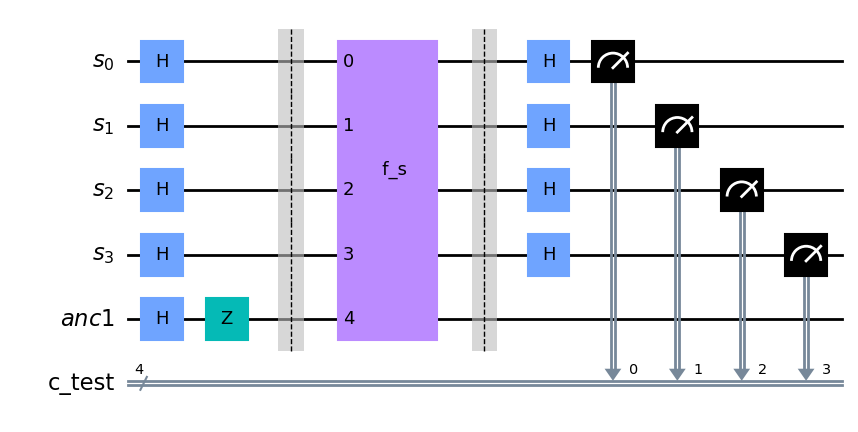
\includegraphics[width=0.8\textwidth]{TFG/imagenes/BV_circuito.png}
    \caption{Circuito, algoritmo BV para s de longitud 4}
    \label{Fig:CircuitoBV}
 \end{figure}

 Detallemos brevemente los elementos principales de este circuito:
 \begin{itemize}
     \item \textbf{Qubits}: Se representan en las primeras lineas, cada uno en una línea distinta. El circuito de la figura 2.2 se compone de 5 qubits. Entre ellos vemos un qubit llamado \textit{anc1}, que es un qubit ancilla con un estado inicial conocido. Algunas veces este qubit auxiliar nos servirá como apoyo para realizar operaciones o almacenará el resultado. Se debería seguir el siguiente esquema para que sea invertible si vemos $U$ como oráculo:
     
     \begin{center}$\Qcircuit @C=1em @R=.7em {\lstick{|x\rangle} & \multigate{1}{U} & \qw & \rstick{|x\rangle} \\ \lstick{|y\rangle} & \ghost{U} & \qw & \rstick{|y \oplus U_{x}\rangle}}$ \end{center}
     
     \vspace{5pt}
     
     \item \textbf{Bits clásicos}: Se representan en la ultima fila, todos juntos. Podemos ver el número, en este caso 4, que nos indica el número de bits clásicos que tenemos.
     
     \item \textbf{Puertas para un qubit}: Podemos observar puertas ya conocidas como Hadamard, Z o la medición que vemos como cae hacia el cable de bits clásicos indicando en que bit se registra la medición.
     
     \item \textbf{Puerta $f_{s}$}: Como ya mencionamos anteriormente puede haber puertas que se apliquen a varios qubits, en este caso tenemos la puerta, o bloque, que replica la función del problema de Bernstein-Vazirani. Dentro de esta puerta tenemos puertas más pequeñas como las presentadas anteriormente en este mismo apartado. En particular, $f_{s}$ tiene puertas CNOT. En diversos algoritmos, se representa esta puerta como un bloque debido a que la podemos entender como un oráculo, del que no sabemos como funciona internamente.
     
     \item \textbf{Barreras}: Nos sirven como apoyo para visualizar el algoritmo y poder separar en secciones.
 \end{itemize}
 
\subsection{Simulaciones y ruido} 
 Una vez que ya hemos visto las puertas que podemos usar en un circuito cuántico, así como un ejemplo del mismo, veamos una introducción a las distintas opciones para la ejecución. \textit{Qiskit} traduce a bajo nivel a \textit{qasm}, que es lo que se va a ejecutar al final. Para ello tenemos las dos opciones siguientes\footnote{\url{https://qiskit.org/documentation/qc_intro.html}}: 
 
 \begin{itemize}
     \item \textbf{Simulación}, en nuestro caso con los simuladores de IBM. Esta posibilidad nos va a ofrecer una simulación teórica de lo que ocurre en nuestro circuito. Será ejecutado a través de un simulador de IBM y nos va a permitir obtener resultados con seguridad y sin ningún problema asociado de errores o ruido. Hay que entender que las simulaciones van a tener una limitación debido a la dimensión de las matrices con las que estamos tratando, ya que el coste es exponencial.
     
     \item \textbf{Ordenador cuántico}, utilizaremos los ordenadores de IBM. La tecnología para la creación de ordenadores cuánticos más fieles sigue avanzando. Esta intenta mitigar los errores que tiene cada operación, así como los errores relacionados con el ruido del entorno que influyen en el estado del sistema modificándolo. Cada ordenador tiene su propia estructura y sus estudios sobre los errores que se cometen en cada qubit, así como calibraciones. Se puede ver en la figura 2.3, los errores de cada qubit así como la estructura del ordenador, además de observar que no todos los qubits tienen relación entre sí, por ejemplo, los qubit 2 y 15 no tienen relación. Qiskit analizará el circuito que le proponemos y lo adaptará a la arquitectura del sistema elegido para la ejecución, con el objetivo de minimizar los errores cometidos.
     
 \end{itemize}
 \vspace{10pt}



 Ambas opciones utilizan el mismo mecanismo, repiten el proceso tantas veces como les sea requerido y muestran la frecuencia acumulada de los resultados (mediciones) o directamente las probabilidades sobre el número total de ejecuciones. \newline



 Veamos un ejemplo para entender la diferencia de resultados de utilizar un opción u otra. Para ello vamos a usar los resultados del circuito presentado en la figura \ref{Fig:CircuitoBV} del algoritmo de Bernstein-Vazirani que se presentará en el siguiente capítulo. Este algoritmo nos debería dar un resultado único, pero veamos lo que ocurre. \newline


Se puede observar en la figura \ref{FIG:ComparacionRealSim} la diferencia entre la simulación teórica (a) y la ejecución con el sistema ibmq\_lima (b). Nuestra simulación nos ha dado únicamente el resultado querido, pero al ejecutarlo en sistema cuántico nos ha dado una variedad de resultados, aunque no todos los posibles. Si bien es cierto que el más probable, con suficiente diferencia, es idéntico al obtenido con la simulación. Cabe destacar de la figura \ref{sFig:Comp_b} que los de mayor probabilidad, una vez eliminada la solución, son aquellos en los cuales solo varía 1 dígito y por el contrario, el complementario binario no ha aparecido como resultado en ninguna de las ejecuciones realizadas.

  \begin{figure}[H]
    \centering
    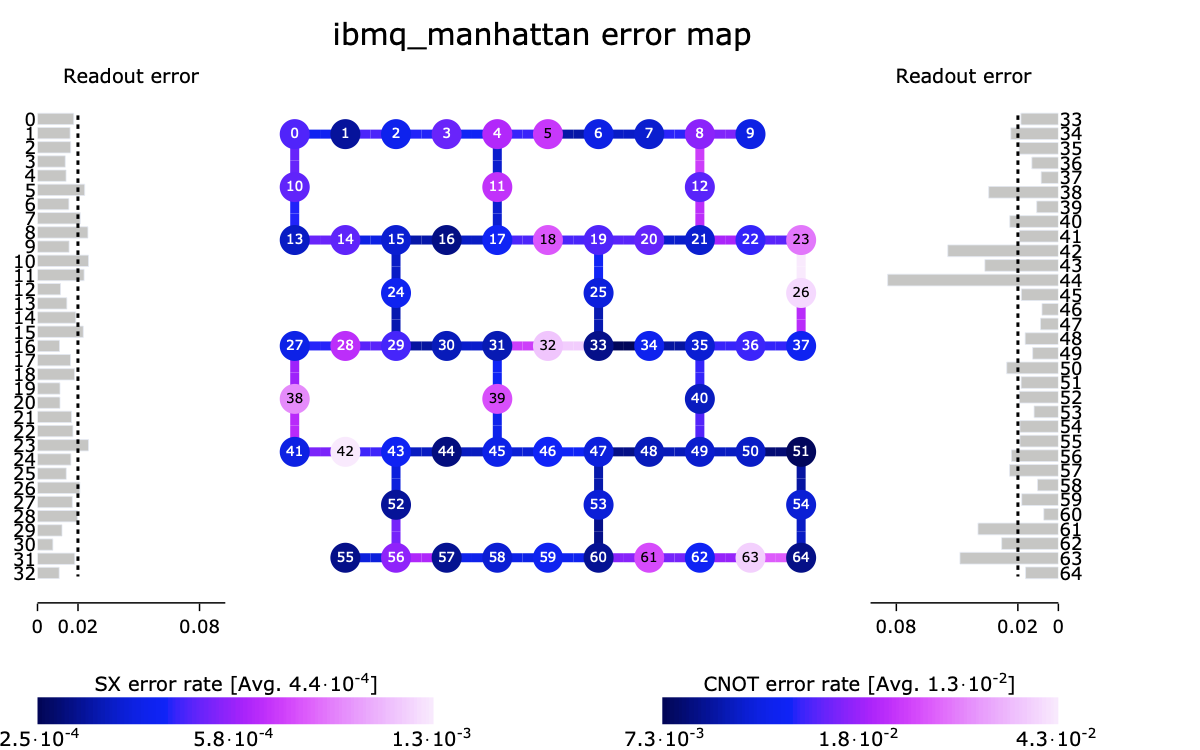
\includegraphics[width=\textwidth]{TFG/imagenes/system_error_manhattan.png}
    \caption{Mapa de errores del ibmq\_manhattan} 
    \label{FIG:MapaErrores}
 \end{figure}

 \vspace{20pt}

\begin{figure}[H]
    \centering
    \begin{subfigure}[H]{0.49\textwidth}
        \centering
        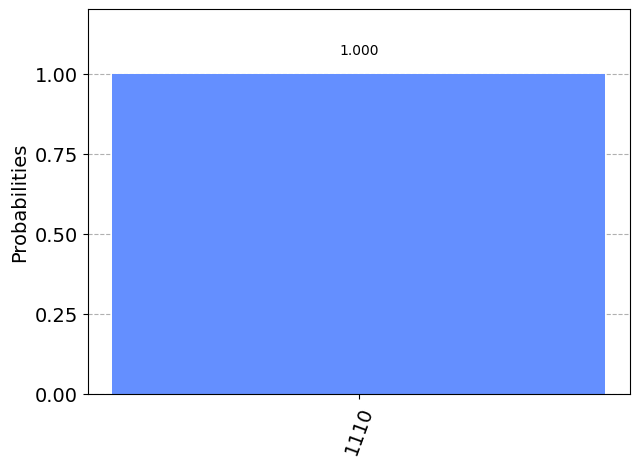
\includegraphics[width=\textwidth]{TFG/imagenes/BV_simulación.png}
        \caption{Simulación}
        \label{sFig:Comp_a}
    \end{subfigure}
    \hfill
    \begin{subfigure}[H]{0.49\textwidth}
        \centering
        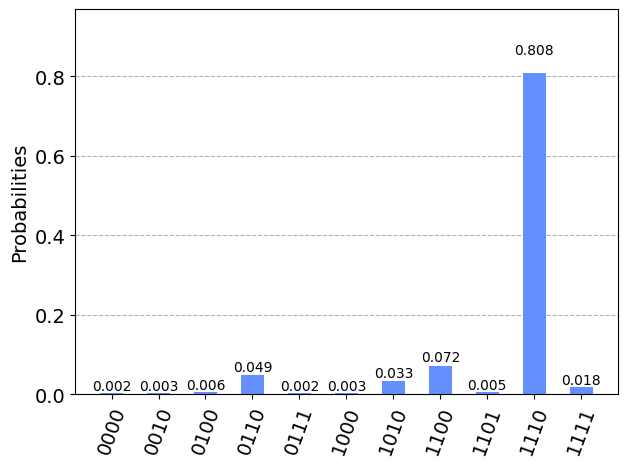
\includegraphics[width=\textwidth]{TFG/imagenes/BV_ruido.png}
        \caption{Sistema cuántico}
        \label{sFig:Comp_b}
    \end{subfigure}
        \caption{Diferencias en resultados de ejecución del algoritmo de Bernstein-Vazirani}
    \label{FIG:ComparacionRealSim}
 \end{figure}

Para acabar con esta sección, como curiosidad y por completitud, hemos mencionado antes que \textit{Qiskit} traduce a \textit{qasm} a la hora de ejecutar. La función utilizada en \textit{Qiskit} para ensamblar el programa es \textit{assemble} que devuelve un objeto de clase \textit{QasmQobj} \footnote{\url{https://qiskit.org/documentation/stubs/qiskit.compiler.assemble.html}}. El código que utilizaría \textit{Qiskit} para la ejecución del circuito presentado anteriormente lo podemos encontrar en el trabajo generado en el sistema cuántico de IBM\footnote{\url{https://quantum-computing.ibm.com/}}. Además, vamos a poder observar en la Figura \ref{FIG:IBMCircBV} el circuito transformado acorde a las puertas de las que dispone el sistema cuántico preparado para la ejecución. Este circuito es el análogo a la Figura \ref{Fig:CircuitoBV} con resultados en la Figura \ref{sFig:Comp_b}.\newline

\begin{figure}[H]
    \centering
    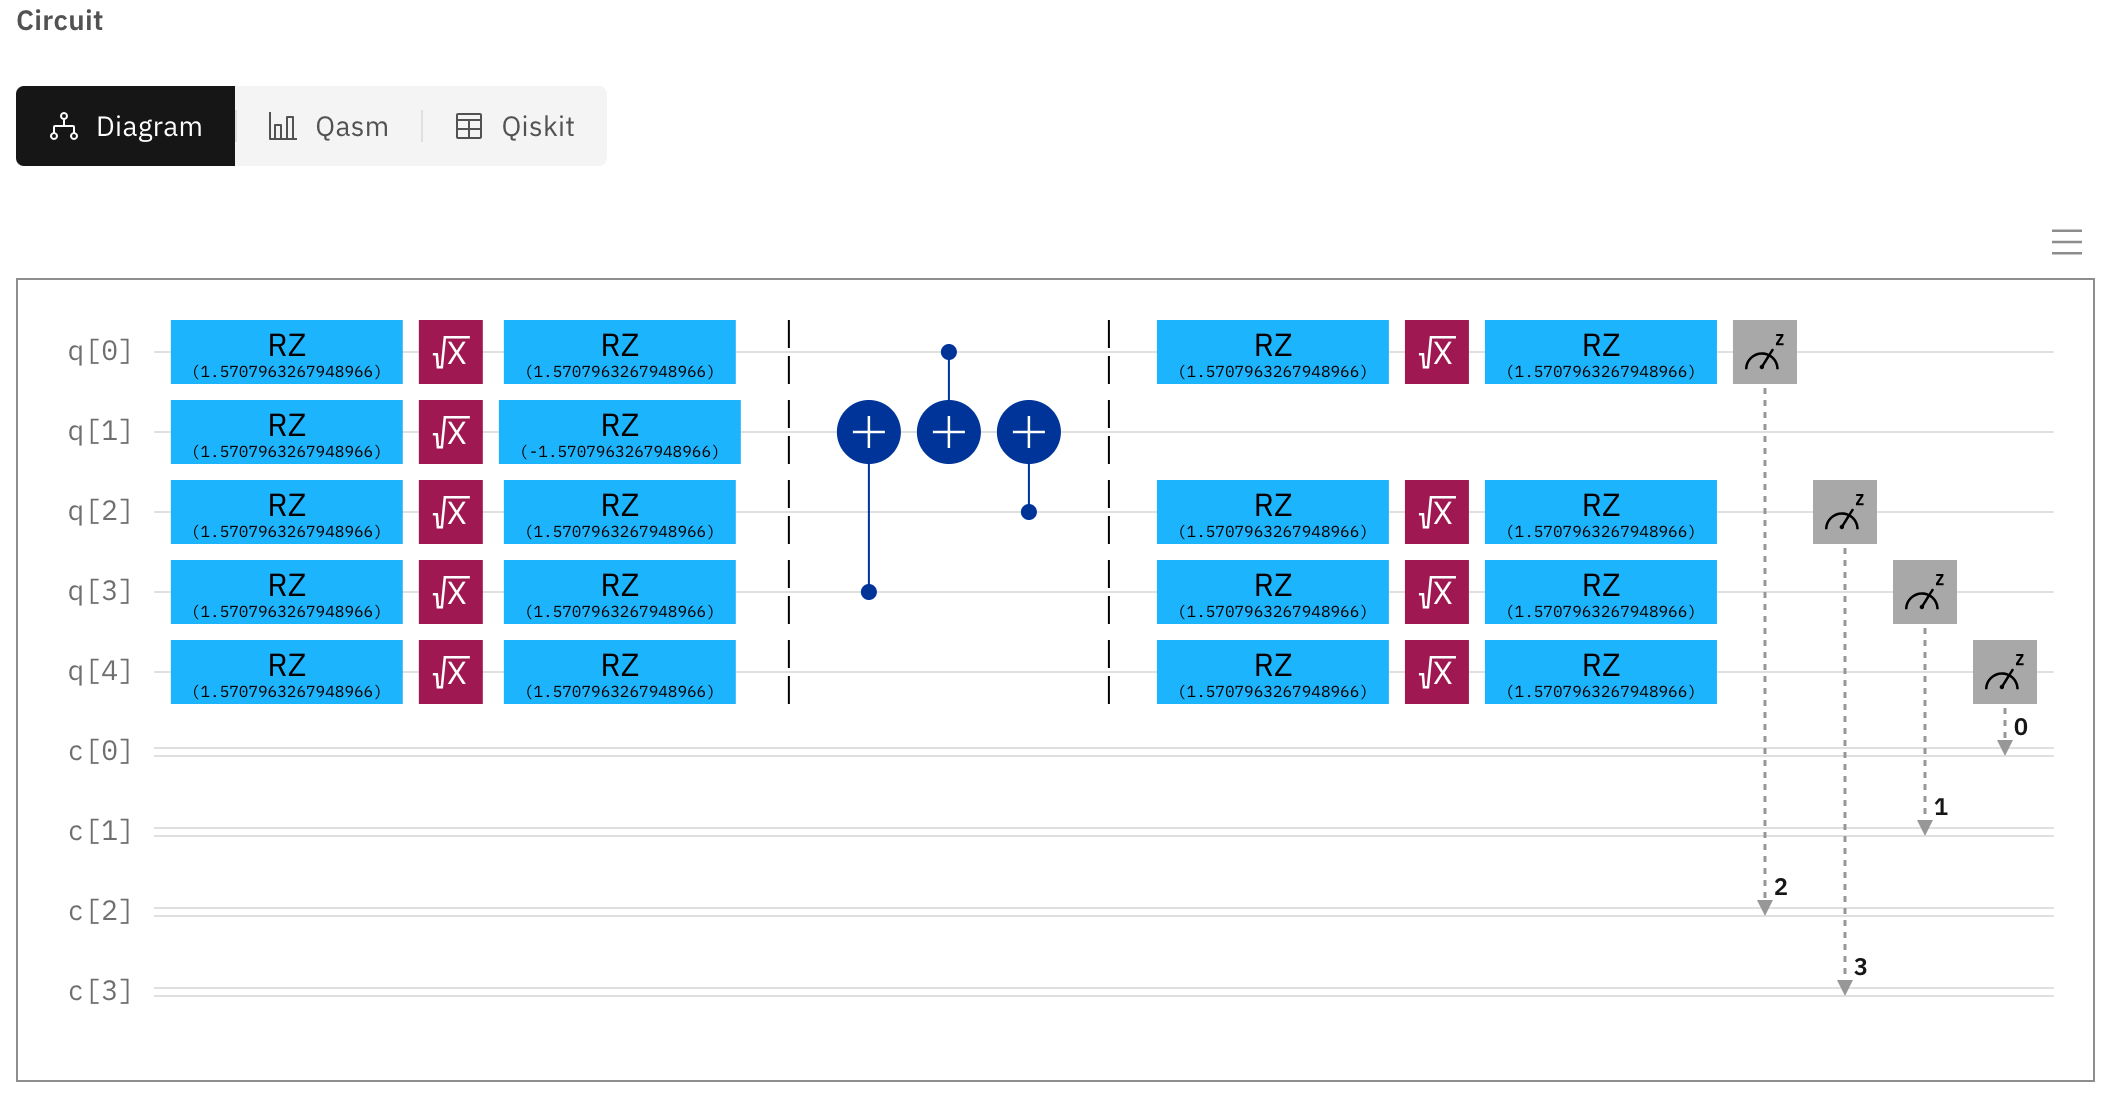
\includegraphics[width=0.7\textwidth]{TFG/imagenes/IBMCircuitBV.png}
    \caption{Circuito del sistema ibmq\_lima para BV, Figura 2.2} 
    \label{FIG:IBMCircBV}
 \end{figure}


\section{Propiedades Metamórficas / \textit{Testing} metamórfico}
\label{Sec2.4:Metamorfico}

Informalmente entendemos como propiedad metamórfica, en adelante MR del inglés \textit{metamorphic rule}, aquella que podemos derivar de forma lógica de una definición o especificación. Empecemos con un ejemplo para ponernos en situación, nos vamos a fijar en la función seno, $f(x)=sin(x)$.\newline


La definición que aprendemos cuando empezamos a ver trigonometría es que el seno es la proporción entre el cateto opuesto y la hipotenusa en un triángulo rectángulo. Teniendo esta imagen la cabeza es muy fácil darse cuenta que $sin(x)=sin(x + 2\pi)=sin(\pi-x)$. Estas son dos propiedades metamórficas de la función seno. \newline

Veamos ahora que es lo que consideramos formalmente una MR y como llegamos a los pasos de testing metamórfico, en adelante MT del inglés \textit{metamorphic testing}\cite{AR:MTmain:2008}:\newline

\begin{itemize}
    \item \textbf{Relación metamórfica}, MR: Sea $f: X \rightarrow Y$ una función. Se considera que $\mathscr{R} \subseteq X^{n} \times Y^{n}$ es una \textbf{regla metamórfica} si es una relación entre una secuencia de entrada $\langle x_{1},x_{2},...,x_{n}\rangle$ con $n>1$ y sus salidas correspondientes $\langle f(x_{1}),f(x_{2}),...,f(x_{n})\rangle$. Es decir, es una propiedad necesaria de f.
    \item \textbf{\textit{Source/follow-up input}}: Sea $\mathscr{R}$ una relación metamórfica y sea $\langle x_{1},x_{2},...,x_{k}\rangle$ la secuencia original con sus respectivos resultados. Denotaremos como \textbf{\textit{source input}} a   $\langle x_{1},x_{2},...,x_{k}\rangle$  los cuales son datos definidos o caracterizados, es decir, ya conocidos. A su vez, podemos generar $\langle x_{k+1},x_{k+2},...,x_{n}\rangle$, los cuales están construidos en base a la entrada original e incluso a la salida de esta. A esta secuencia la llamaremos \textbf{\textit{follow-up input}}.
    \item \textbf{Grupo metamórfico de entrada}: Llamaremos \textbf{grupo metamórfico de entrada} a la secuencia definida por \textit{source} y \textit{follow-up input}, es decir, $\langle x_{1},x_{2},...,x_{k},x_{k+1},...,x_{n}\rangle$.
    \item \textbf{\textit{Testing} metamórfico}, MT\label{Def:MT}: Sea $f$ la función objetivo, $P$ una implementación de $f$ y $\mathscr{R}$ una regla metamórfica de $f$.
    
    Para realizar \textbf{\textit{testing} metamórfico} sobre $P$ seguiremos los siguiente pasos:
    \begin{itemize}
        \item Definimos $\mathscr{R}'$ reemplazando $f$ por $P$ en $\mathscr{R}$.
        \item Dado el \textit{source input}, generamos sus salidas según $P$, construimos a partir de estos el \textit{follow-up input} $\langle x_{k+1},...,x_{n}\rangle$, y obtenemos $\langle P(x_{k+1}),...,P(x_{n})\rangle$.
        \item Estudiamos los resultados obtenidos respecto a $\mathscr{R}'$. Si $\mathscr{R}'$ no se satisface entonces podemos afirmar que $P$ no es correcto.
    \end{itemize}
\end{itemize}

La estrategia presentada anteriormente para MT, será la que se siga en la implementación de las propiedades que se obtendrán a lo largo de este documento. \newline

Para finalizar con esta introducción vamos a revisar brevemente un par de ventajas y retos que presenta el camino que estamos tomando para probar la corrección, o más bien la no corrección, de un algoritmo. \newline

\textbf{Ventajas}:
\begin{itemize}
    \item \textbf{Simplicidad}. El concepto e interpretación de una MR es bastante simple en comparación con otros conceptos que se utilizan dentro del campo del testing. Se ha visto en estudios, que incluso gente con poca experiencia, podrían utilizar estas técnicas en relativamente poco tiempo de forma efectiva.\cite{AR:MTmain:2008} \cite{Note:MT55} \cite{Note:MT73}
    \item \textbf{Facilidad en la implementación}. Si partimos de la ventaja anterior como es la simplicidad de la definición, podemos continuar que la implementación de este test es prácticamente seguir los pasos explicados en la definición de \hyperref[Def:MT]{MT}.
\end{itemize}

\vspace{10pt}

\textbf{Retos}:
\begin{itemize}
    \item \textbf{Generación efectiva de los grupos metamórficos de entrada}. Aun se sigue estudiando que garantías tenemos en la efectividad que puede tener la elección del grupo metamórfico de entrada en la demostración de la corrección de un algoritmo y en particular, la forma en la que obtenemos nuestro \textit{source input}, ya que \textit{follow-up input} se genera a partir de esta. Al fin y al cabo nuestro objetivo es maximizar la identificación de errores o defectos en $P$.
    
    \item \textbf{Estructura del MT}. Debido a la gran variedad de MR, aun no hay un acuerdo sobre una estructura definida y formal que nos proporcione seguridad en nuestra pruebas y englobe a todas las posibilidades que tenemos dentro de las MR. Aunque, si bien es cierto, ya ha ayudado a identificar diversos errores en sistemas muy estudiados con otros métodos de \textit{testing}, como por ejemplo los compiladores GCC y LLVM de C, en los cuales encontró más de 100 fallos.\cite{AR:MTmain:2008} \cite{Note:MT50} \cite{Note:MT51} \cite{Note:MT78}
\end{itemize}

Los retos de MT pueden ser una buena base para todo el trabajo futuro que se puede realizar en este campo y las posibilidades que este nos puede ofrecer. Trataremos en más profundidad estás posibilidades en la \hyperref[Sec5.2:Futuro]{sección 5.2} de posibles trabajos futuros.



